\section{Введение}

\begin{frame}
\frametitle{Введение}
\begin{figure}
    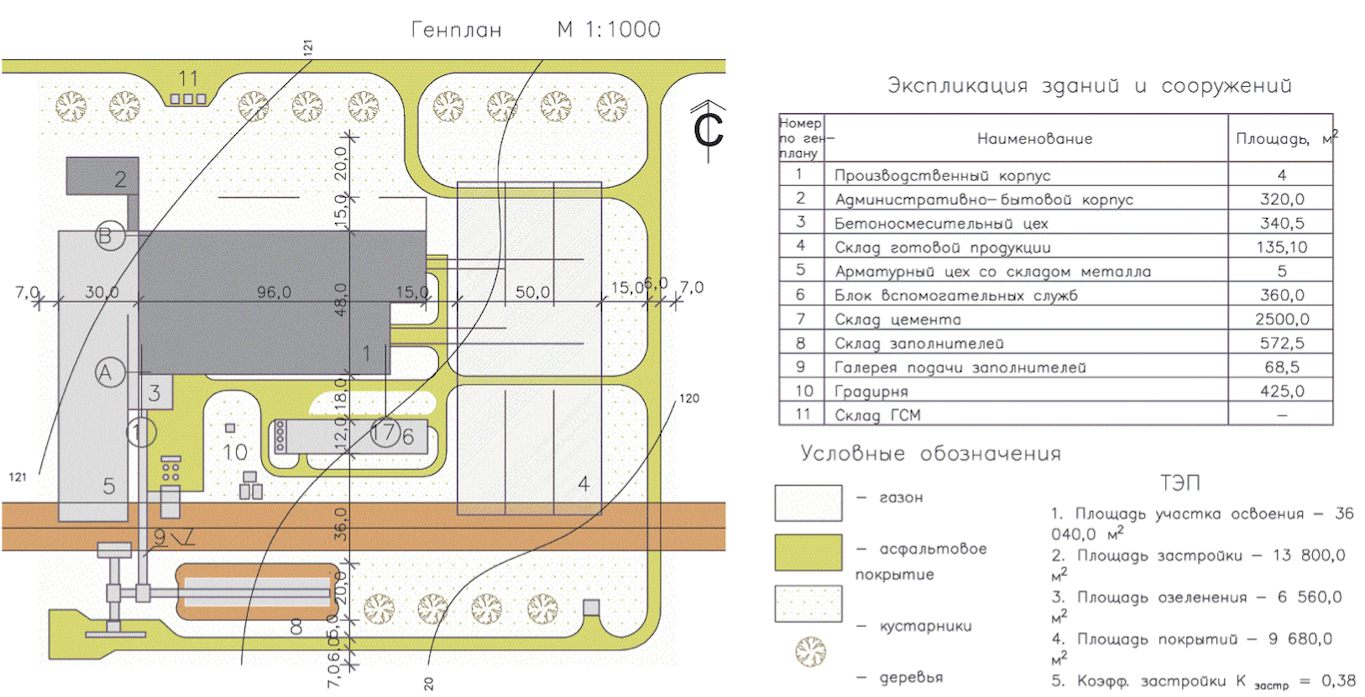
\includegraphics[scale=.5]{pictures/common/site_plan}
    \caption{Пример генерального плана площадного объекта}
\end{figure}
\end{frame}


\section{Постановка задачи}

\begin{frame}
\frametitle{Цель работы}
Упрощение процесса проведения научных изысканий
в области автоматического формирования генеральных планов площадных объектов
путём создания программного компонента.
\end{frame}


\begin{frame}
\frametitle{Задачи}
\begin{enumerate}
    \item сбор и анализ требований пользователей системы,
    \item анализ возможной нагрузки и вариативности используемых данных,
    \item формирование системной и программной архитектуры,
    \item реализация полученного решения.
\end{enumerate}
\end{frame}
